\documentclass{article}
\usepackage{listings} % For code formatting
\usepackage[utf8]{inputenc}  % For encoding support
\usepackage{amsmath}         % For mathematical formatting
\usepackage{graphicx}        % For including images
\usepackage{xcolor}
\usepackage[a4paper, left=0.5in, right=0.5in, top=0.5in, bottom=0.5in]{geometry}  % Adjust margins here
\usepackage{tcolorbox}
\usepackage{palatino}  % Use Inconsolata font (or replace with your choice)

% Define colors
\definecolor{codebg}{RGB}{240, 240, 240}  % Light gray background
\definecolor{framecolor}{RGB}{100, 100, 100}  % Dark gray frame
\definecolor{titlebg}{RGB}{30, 30, 30}  % Dark title background
\definecolor{titlefg}{RGB}{255, 255, 255}  % White title text

% Custom lstset
\lstset{
    language=C++,                    
    basicstyle=\ttfamily\footnotesize\fontfamily{zi4}\selectfont, % Use Inconsolata
    keywordstyle=\bfseries\color{blue},        
    commentstyle=\itshape\color{gray},        
    stringstyle=\color{red},          
    numbers=left,                     
    numberstyle=\tiny\color{blue},    
    frame=single,                     
    breaklines=true,                   
    captionpos=b,                      
    backgroundcolor=\color{codebg},  % Light gray background
    rulecolor=\color{framecolor},    % Dark frame
    tabsize=4                         
}

% Custom command to add a styled heading
\newtcbox{\codebox}{colback=titlebg, colframe=titlebg, colupper=titlefg, 
  boxrule=0pt, arc=5pt, left=5pt, right=5pt, top=3pt, bottom=3pt}

\title{Parallel Programming Assignment 2 \\ Parallel Delta Stepping Algorithm Implementation and Experimentation using MPI}
\author{Ayush Raina, 22148}
\date{\today}

\begin{document}

\maketitle
\subsection*{Delta Stepping Algorithm}

Delta-Stepping is a parallel algorithm for solving the \textbf{Single-Source Shortest Path (SSSP)} problem, particularly effective on graphs with both \textbf{light} and \textbf{heavy} edges. It was introduced by Ulrich Meyer and Peter Sanders to achieve high performance on shared and distributed memory systems by exploiting parallelism in edge relaxation.

\subsubsection*{Problem Definition}
Given a graph \( G = (V, E) \), where \( V \) represents the set of vertices and \( E \) represents the set of weighted edges with non-negative weights, and a source vertex \( s \in V \), the objective of the algorithm is to compute the shortest path distance \( d(v) \) from the source \( s \) to every vertex \( v \in V \).

\subsubsection*{Key Concept: Light and Heavy Edges}
Edges are categorized based on a threshold parameter \( \Delta > 0 \):
\begin{itemize}
    \item \textbf{Light Edges}: Edges with weight \( w(e) \leq \Delta \)
    \item \textbf{Heavy Edges}: Edges with weight \( w(e) > \Delta \)
\end{itemize}

This distinction allows the algorithm to process light edges concurrently while deferring the processing of heavy edges, thereby enhancing parallel efficiency.

\subsubsection*{Algorithm Workflow}
\begin{enumerate}
    \item \textbf{Initialization:}
    \begin{itemize}
        \item Set the distance to the source vertex \( s \) as \( d(s) = 0 \), and to all other vertices as infinity \( d(v) = \infty \) for \( v \neq s \).
        \item Initialize a collection of buckets \( B[i] \), where each bucket stores vertices with distances in the range:
        \[
        B[i] = \{ v \mid i \times \Delta \leq d(v) < (i + 1) \times \Delta \}
        \]
    \end{itemize}
    
    \item \textbf{Bucket Processing Loop:}
    \begin{itemize}
        \item While there are non-empty buckets:
        \begin{itemize}
            \item Extract and process the \textbf{smallest non-empty bucket} \( B[i] \).
            \item Relax \textbf{light edges} of vertices in the bucket and update distances.
            \item Move vertices to appropriate future buckets based on updated distances.
        \end{itemize}
    \end{itemize}
    
    \item \textbf{Handling Heavy Edges:}
    \begin{itemize}
        \item After all light edges are processed, relax heavy edges.
        \item If the distance of a vertex changes, place it in the appropriate bucket.
    \end{itemize}
    
    \item \textbf{Termination:}
    \begin{itemize}
        \item The algorithm terminates when all buckets are empty, ensuring all shortest paths are computed.
    \end{itemize}
\end{enumerate}

\subsubsection*{Mathematical Formulation}
For a vertex \( v \) with current distance \( d(v) \), when relaxing an edge \( (v, u) \) with weight \( w \):

\[
  d(u) = \min(d(u), d(v) + w)
\]

If \( w \leq \Delta \), the edge is considered \textbf{light} and processed immediately. Otherwise, it is \textbf{heavy} and deferred.

\subsubsection*{Parallelization Strategy}
In a distributed-memory setting using MPI, the graph is partitioned across multiple processes. Each process handles a subset of vertices and their outgoing edges. Communication occurs to share updated distances:

\begin{itemize}
    \item \textbf{Local Processing:} Each process updates its local vertices.
    \item \textbf{Exchange Updates:} Use collective operations (e.g., \texttt{MPI\_Alltoallv}) to share changes across processes.
    \item \textbf{Synchronization:} Ensure global consistency via reduction operations.
\end{itemize}

\subsection*{Experimental Setup}
All the experiments are done on teaching cluster provided to us. The graph used in experiementation contains 1,971,281 vertices and 5,533,214 edges with randomly assigned weights $w(e) \in [1, 100]$. We are choosing source vertex to be 0. Following is the execution times for 1,2,4,8,16,32,64 processors along with Speedup and Efficiency for different Delta Values

\begin{table}[h]
    \centering
    \begin{tabular}{|c|c|c|c|c|c|c|c|c|}
        \hline
        \textbf{Delta} & \textbf{1 Proc} & \textbf{2 Proc} & \textbf{4 Proc} & \textbf{8 Proc} & \textbf{16 Proc} & \textbf{32 Proc} & \textbf{64 Proc} \\
        \hline
        1   & 4.503  & 3.515  & 3.100  & 3.026  & 2.939  & 3.467 & 8.079 \\
        5  & 4.536  & 3.523  & 3.091  & 2.825  & 2.947   & 3.399   & 8.108      \\
        10  & 4.530  & 3.631  & 3.090  & 2.908  & 3.053   & 3.412   & 7.903    \\
        20  & 4.507  & 3.536  & 3.042 & 2.892   & 2.990  & 3.421 & 8.117   \\
        30 & 4.493  & 3.619  & 3.121  & 2.942  & 2.983   & 3.434   & 7.930  \\
        40 & 4.500   & 3.525  & 3.120  & 2.938  & 2.973   & 3.490   & 8.353  \\
        50 & 4.504   & 3.538  & 3.186  & 2.965  & 3.000   & 3.420   & 7.992     \\
        60 & 4.507   & 3.516  & 3.185  & 2.928  & 2.916   & 3.583   & 8.651    \\
        70 & 4.498   & 3.455  & 3.096  & 2.877  & 2.971   & 3.563   & 8.428    \\
        80 & 4.536   & 3.459  & 3.064  & 3.042  & 2.922   & 4.855   & 8.156   \\
        90 & 4.505   & 3.440  & 3.259  & 3.032  & 2.945   & 3.570   & 8.059    \\
        100 & 4.511  & 3.543  & 3.148  & 2.955  & 2.964   & 3.376   & 8.425      \\
        \hline
    \end{tabular}
    \caption{Execution times (in seconds) for different processor counts and Delta values}
    \label{tab:execution_times}
\end{table}

In the above table, the execution time for involving more than 1 processor is reported for the processor which took the maximum time. Here are some plots to visualize the above data.

\begin{figure}[h]
    \centering
    \includegraphics[width=0.8\textwidth]{speedup.png}
    \caption{Speedup vs Number of Processors for Different Delta Values}
    \label{fig:speedup}
\end{figure}

\begin{figure}[h]
    \centering
    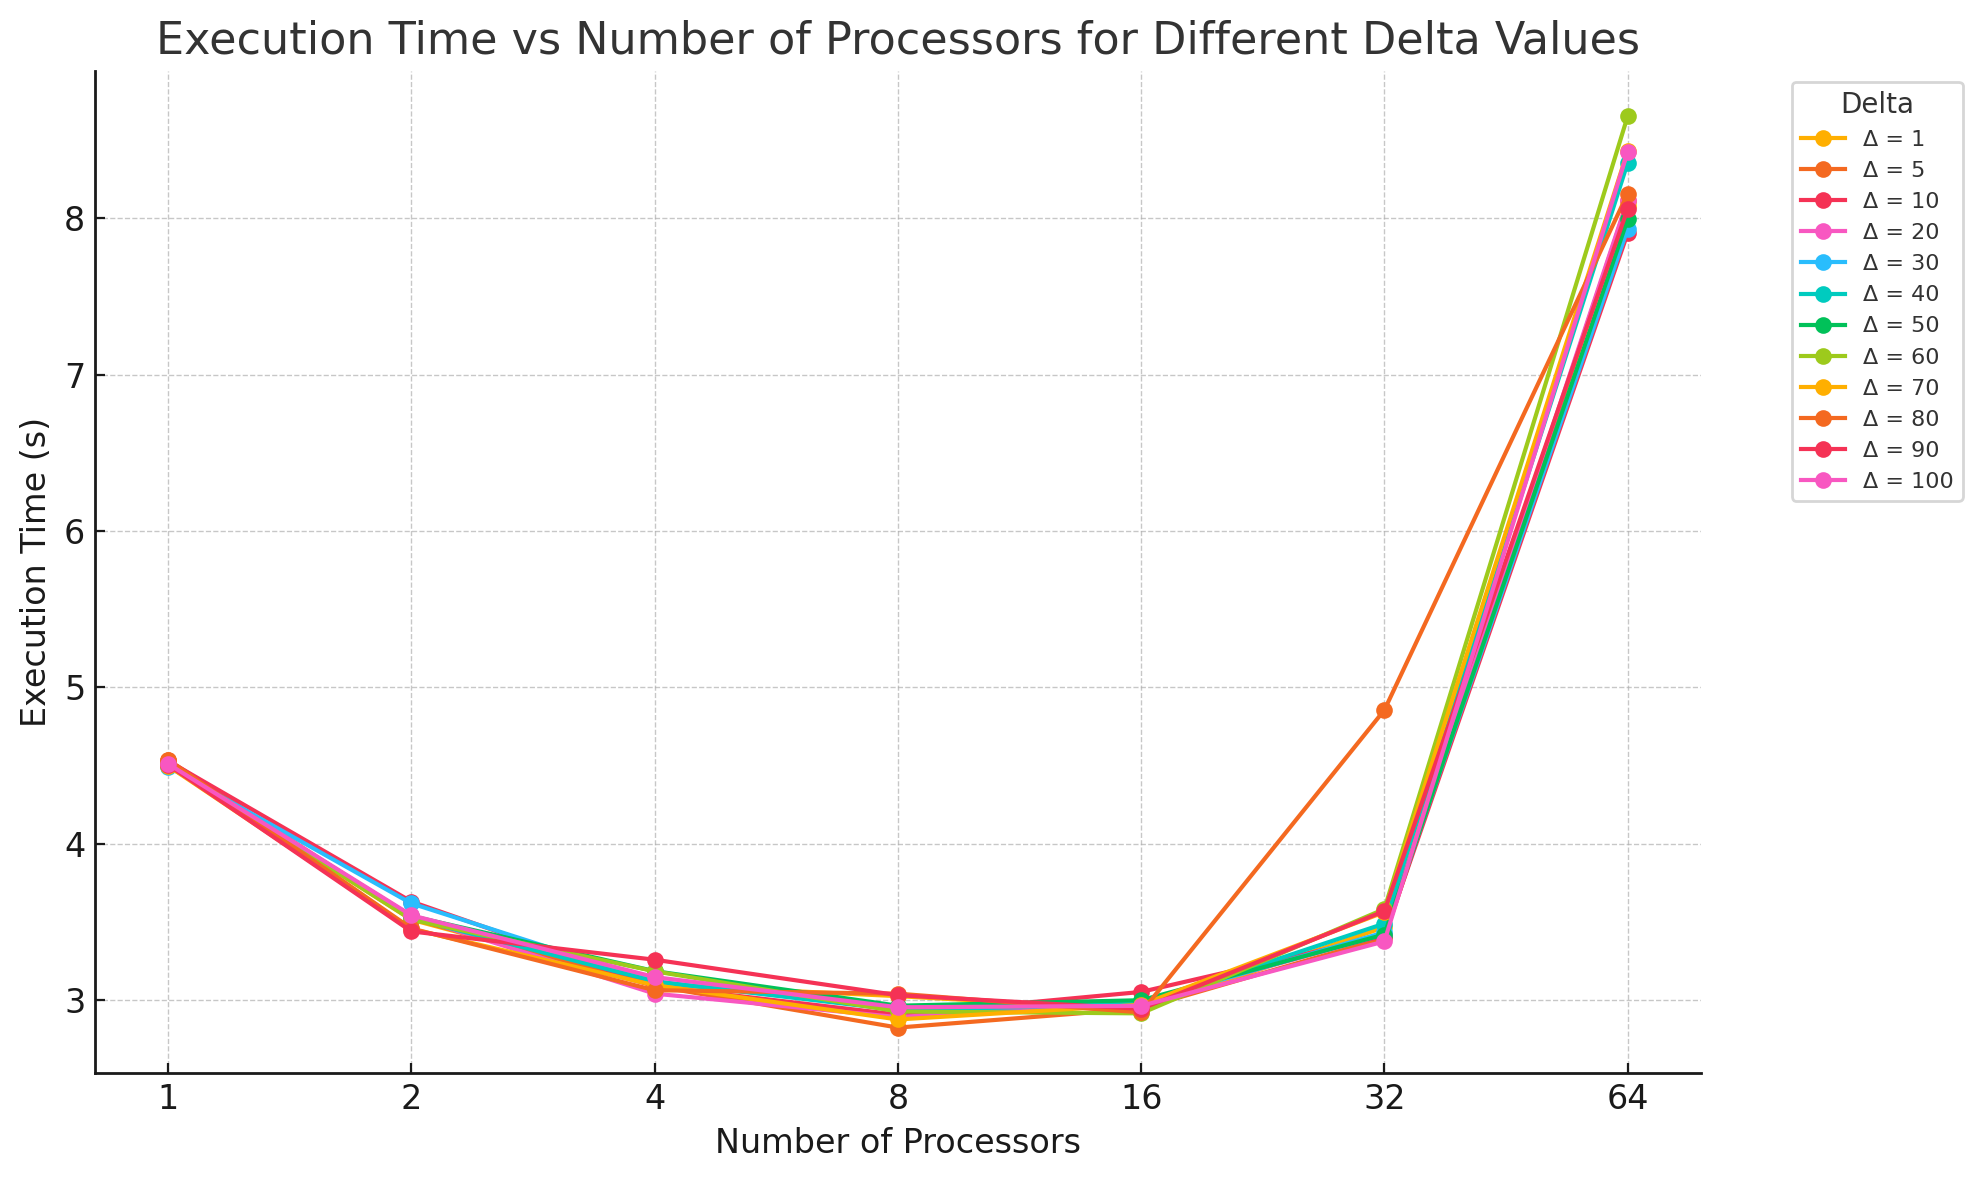
\includegraphics[width=0.8\textwidth]{executionTime.png}
    \caption{Execution Time vs Number of Processors for Different Delta Values}
    \label{fig:efficiency}
\end{figure}

\newpage

\subsection*{Parallel Overhead Calculation}
We can also calculate Parallel Overhead which quantifies extra work incurred due to parallelization - such as communication, synchronization and load imbalance. It is defined as $PO = T_N \times P - T_1$ where $T_N$ is the execution time for N processors and $T_1$ is the execution time for 1 processor. Here is the plot for Parallel Overhead for different Delta Values.

\begin{figure}[h]
    \centering
    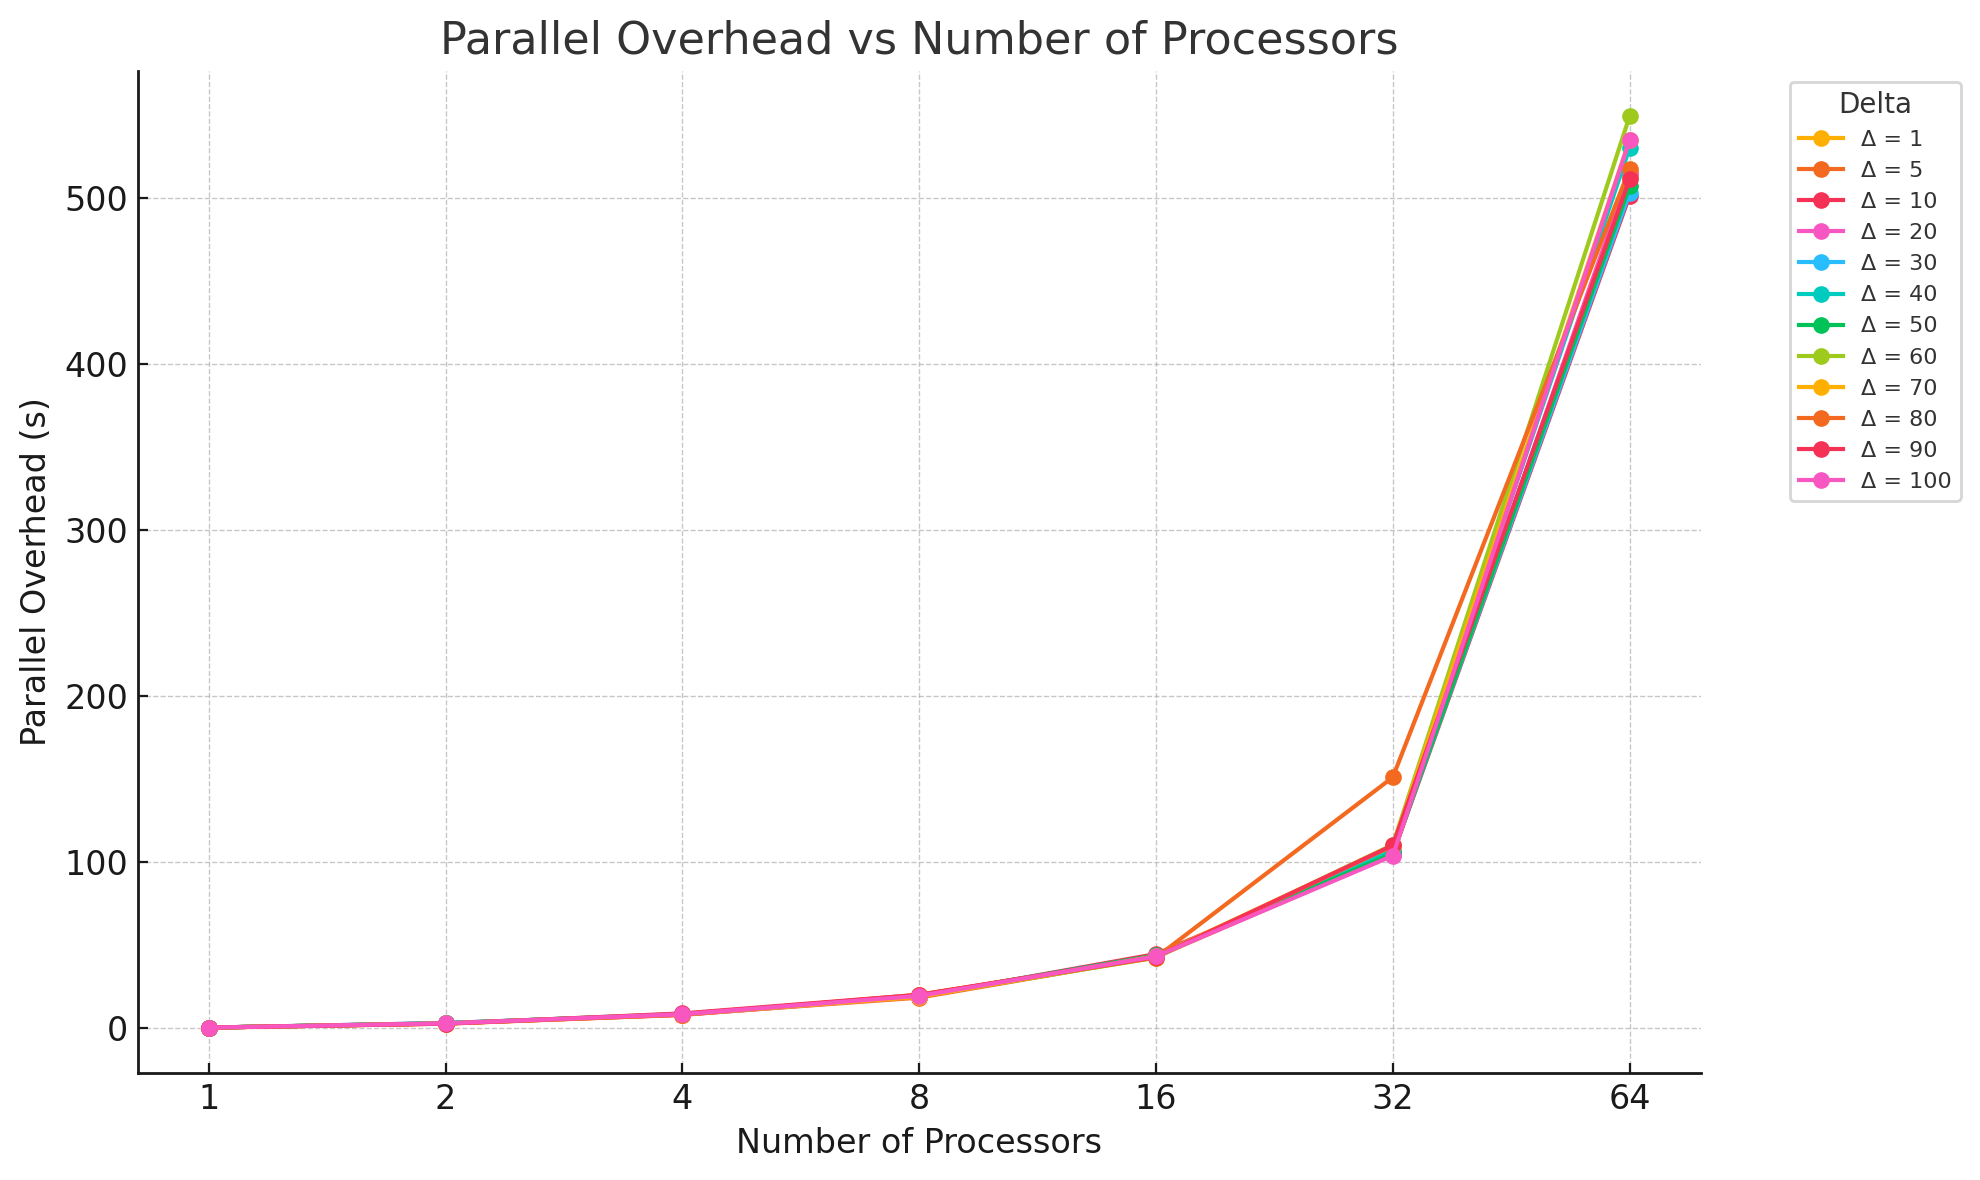
\includegraphics[width=0.8\textwidth]{overhead.png}
    \caption{Parallel Overhead vs Number of Processors for Different Delta Values}
    \label{fig:parallelOverhead}
\end{figure}

One more reason, I think for huge increase in overhead when we move to 64 processor from 32 processors is because the machine in which we are running the code has 32 cores. I tried all these experiments with my 24 core machine also in which same pattern followed. Initially execution time kept decreasing until 16 cores, then if I use \textbf{--oversubscribe} flag to run with 32 and 64 processors, the execution time increased. 

\newpage 

Here is efficiency plot for different Delta Values.
\begin{figure}[h]
    \centering
    \includegraphics[width=0.8\textwidth]{efficiency.png}
    \caption{Efficiency vs Number of Processors for Different Delta Values}
    \label{fig:efficiency}
\end{figure}

From above plot we can see that even we are lowering the execution time till 8 processors, but still the resource utilization is not up to the mark. This is because of communication overheads, synchronization overheads as Delta Stepping Algorithm is a bulk synchronization algorithm, and non trivial programming using MPI. My implementation is around 1000 lines of code and I used \textbf{modulus} operator to distribute the vertices among processors, due to which all processors have got almost equal number of vertices to process. So \textbf{load imbalance} is not an issue, \textbf{communication and synchronization overheads} are the main reasons for low efficiency.

\subsection*{Hybrid Implementation Using Open MP and CUDA}
We implemented the same Delta Stepping Algorithm using Open MP and CUDA. We used Open MP for parallelizing the bucket processing loop and CUDA for parallelizing the edge relaxation step. We used 8 threads for Open MP and 256 threads per block for CUDA.Here is the execution times for different Delta Values.

\begin{table}[ht]
    \centering
    \caption{Execution Times for Different Delta Values (OpenMP + CUDA)}
    \begin{tabular}{|c|c|}
        \hline
        \textbf{Delta Value} & \textbf{Execution Time (s)} \\
        \hline
        1 & 6.1021 \\
        \hline
        5 & 3.4281 \\
        \hline
        10 & 3.3989 \\
        \hline
        20 & 1.5955 \\
        \hline
        30 & 2.4969 \\
        \hline
        40 & 1.5924 \\
        \hline
        50 & 1.3124 \\
        \hline
        60 & 1.3066 \\
        \hline
        70 & 1.61707 \\
        \hline
        80 & 1.5882 \\
        \hline
        90 & 2.2041 \\
        \hline
        100 & 1.3141 \\
        \hline
    \end{tabular}
    \label{tab:delta_timing}

    Assuming Sequential Execution Time (T\_seq): 4.503 seconds
    \begin{equation}
        \text{Speedup} = \frac{T_{seq}}{T_{par}}
    \end{equation}
    and 
    \begin{equation}
        \text{Efficiency} = \frac{\text{Speedup}}{P}
    \end{equation}
    Where $T_{par}$ is the execution time for parallel implementation and $P$ is the number of processors which is 8 in this case.

\end{table}
Here are the plots for speedup, execution times and efficiency for OpenMP + CUDA implementation for different Delta Values.

\begin{figure}[h]
    \centering
    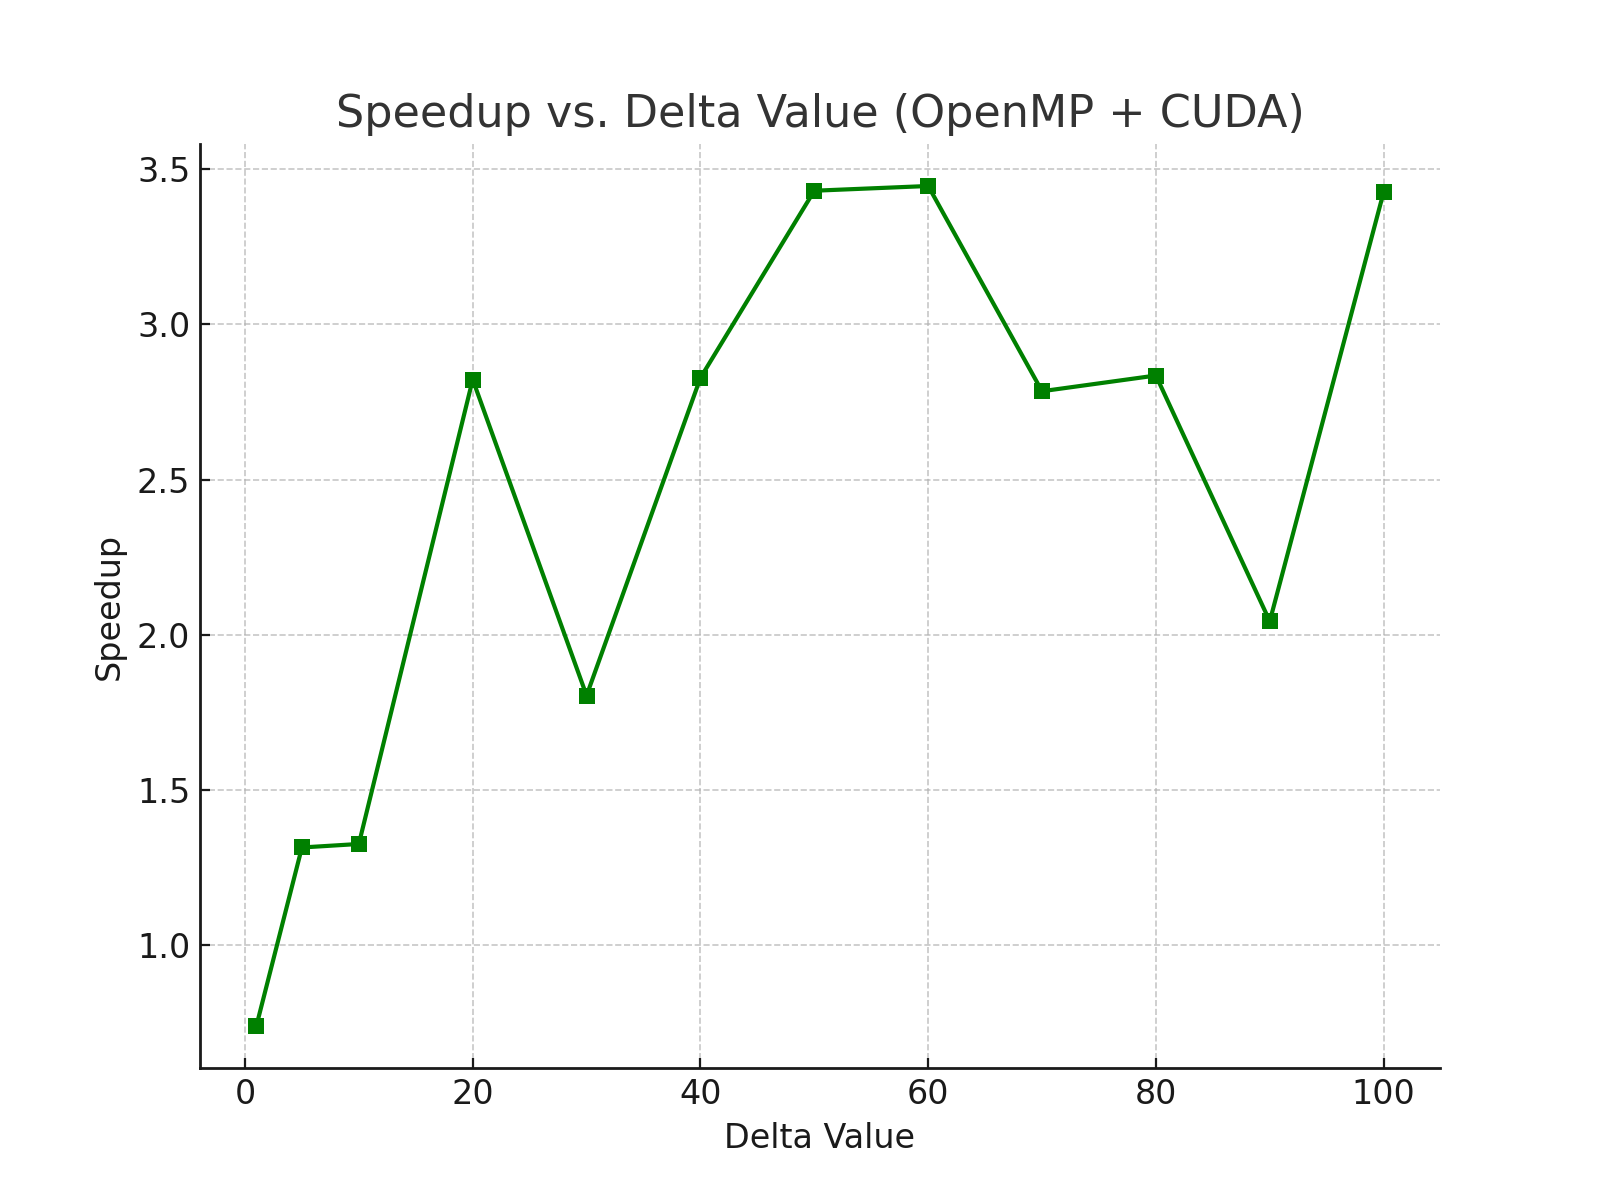
\includegraphics[width=0.4\textwidth]{speedup_vs_delta.png}
    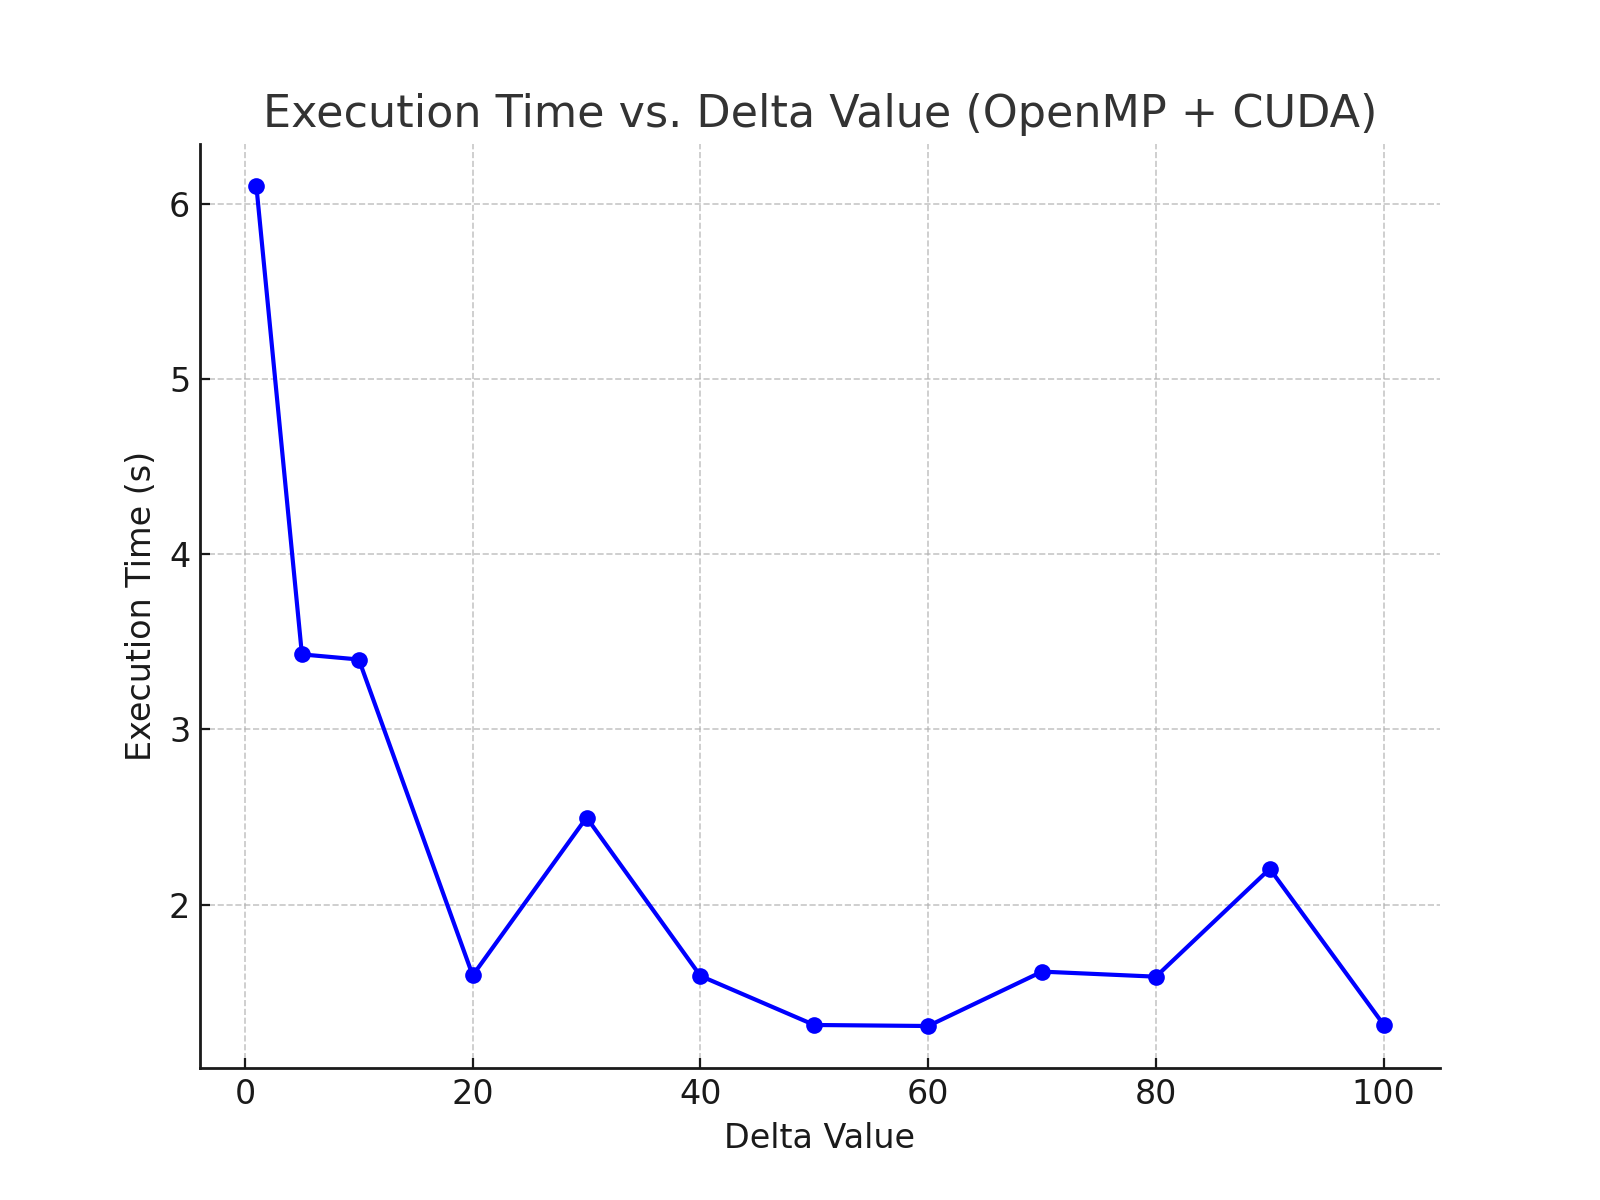
\includegraphics[width=0.4\textwidth]{execution_time_vs_delta.png}
    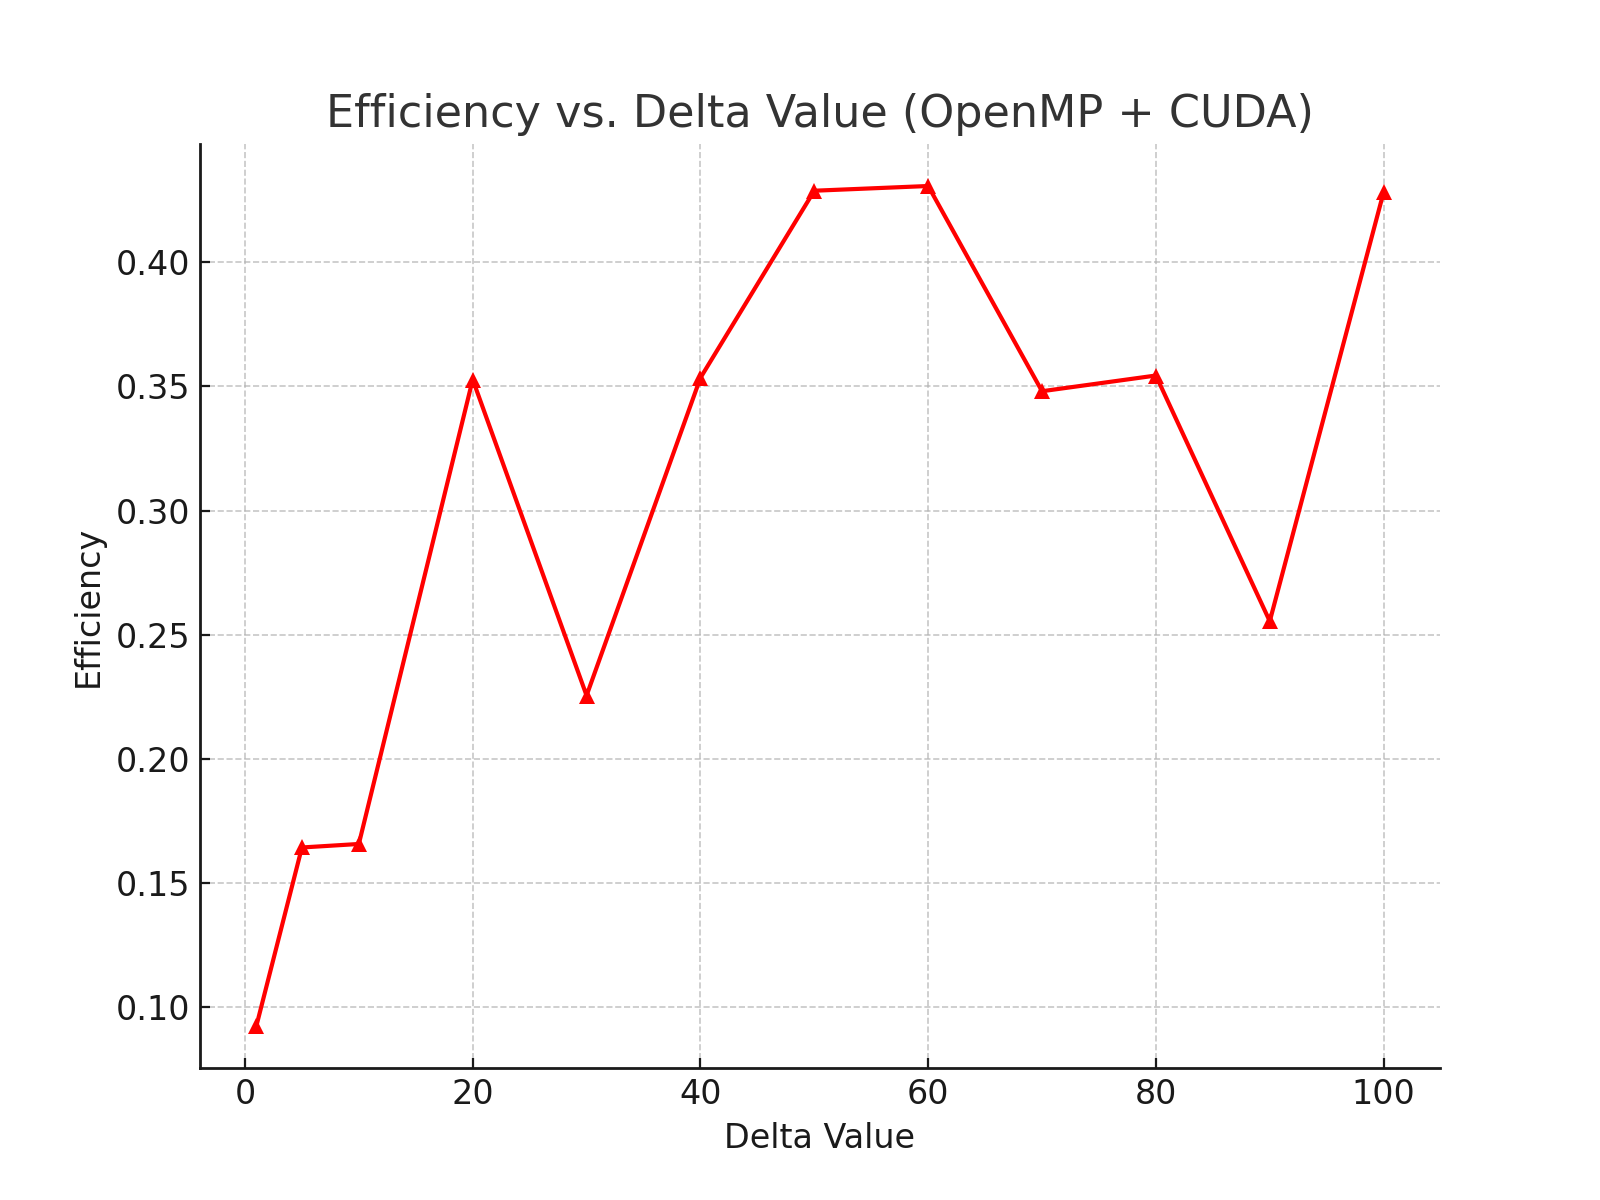
\includegraphics[width=0.4\textwidth]{efficiency_vs_delta.png}
    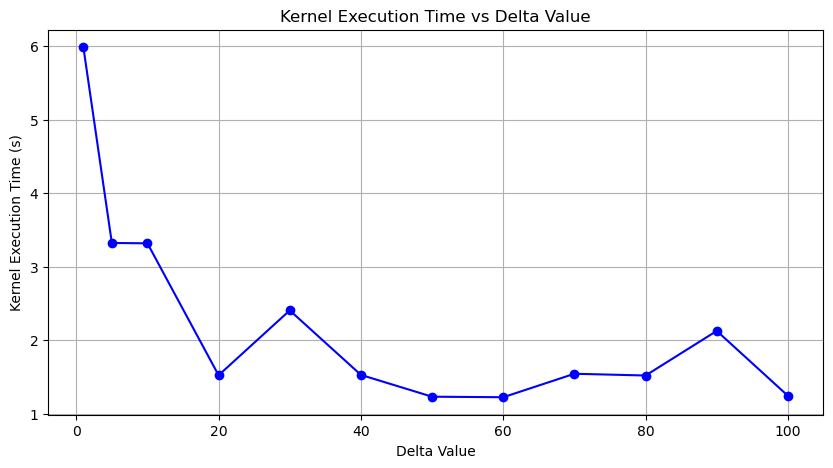
\includegraphics[width=0.4\textwidth]{KernelTime.png}
    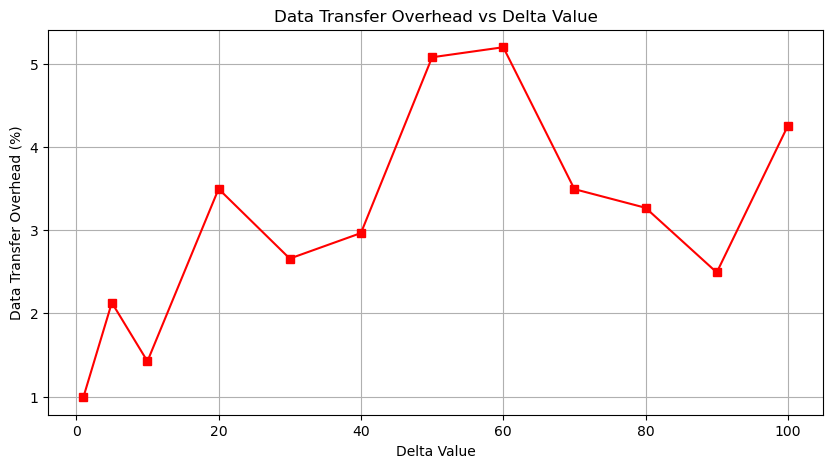
\includegraphics[width=0.4\textwidth]{kernelOverhead.png}

    \caption{Speedup vs Delta Values for OpenMP + CUDA Implementation}
    \label{fig:speedup_openmp_cuda}
\end{figure}


\end{document}
